\documentclass{standalone}
\usepackage{tikz}
\usetikzlibrary{patterns}
\usetikzlibrary{positioning}
\usetikzlibrary{patterns, positioning}
\usetikzlibrary{shapes.misc}
\usepackage[outline]{contour}
\contourlength{1.5pt} 
\usetikzlibrary{calc}
        \usepackage{relsize}
        \tikzset{fontscale/.style = {font=\relsize{#1}}}

\begin{document}
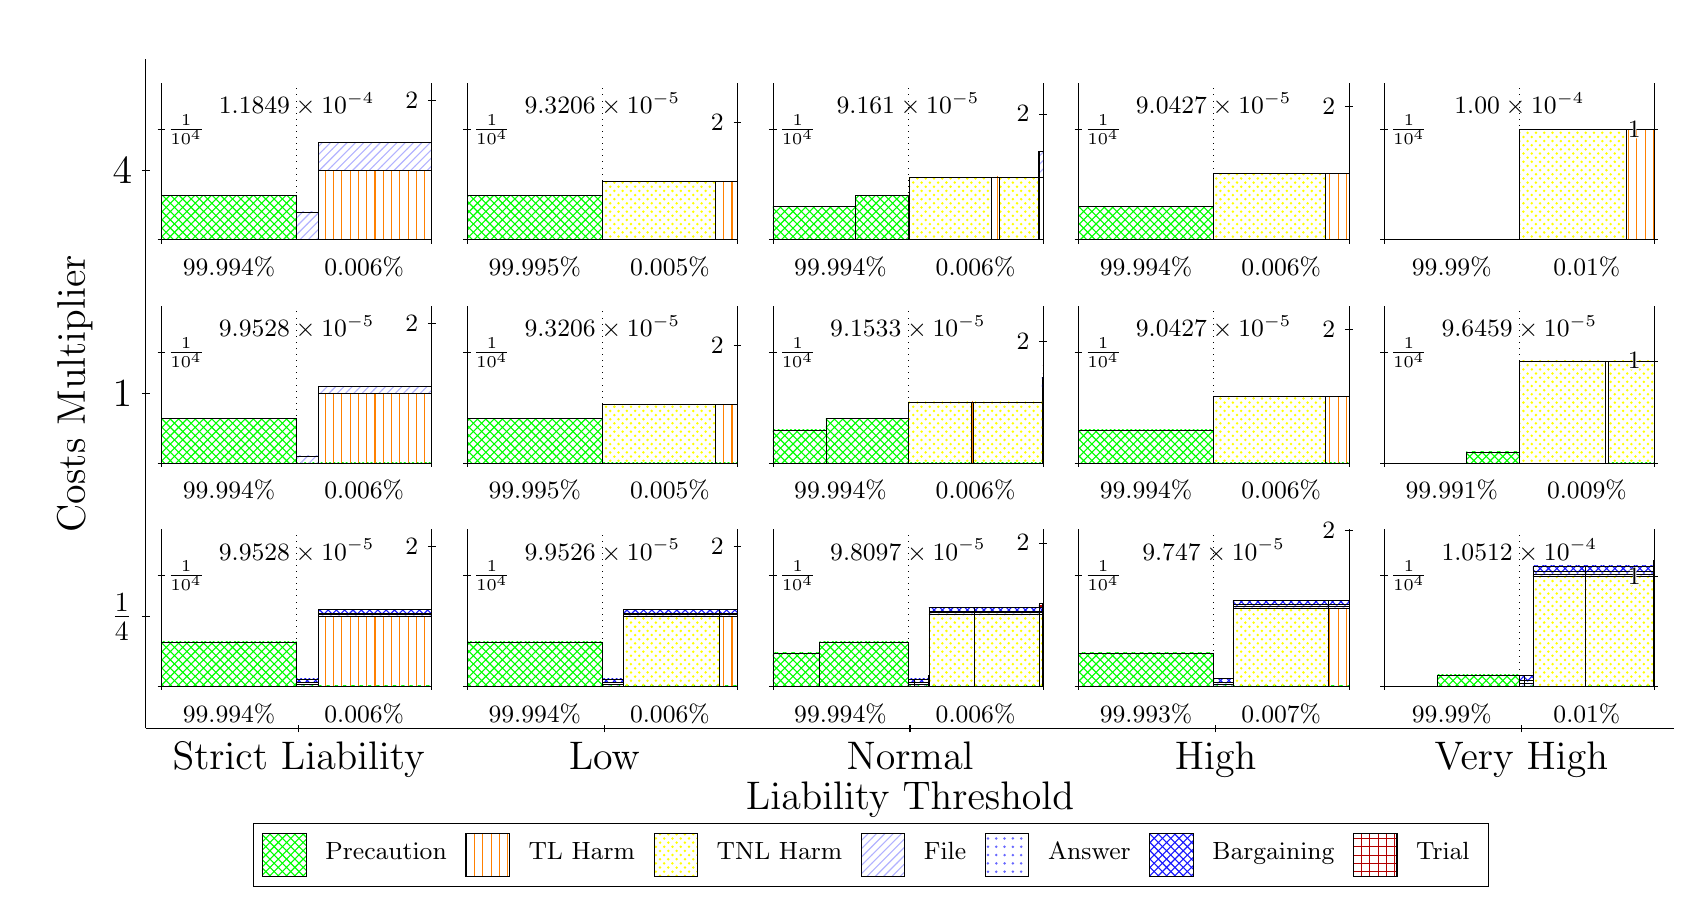
\begin{tikzpicture}
\clip(-0.5,-1.1) rectangle +(20.91,11);
\draw[black] (1,1) -- (1,9.5);
\node[rotate=90, fontscale=2, anchor=center] at (0.1, 5.25) {Costs Multiplier};
\draw[black] (0.95,2.4167) -- (1.05,2.4167);
\node[fontscale=2, anchor=east] at (0.95, 2.4167) {$\frac{1}{4}$};
\draw[black] (0.95,5.25) -- (1.05,5.25);
\node[fontscale=2, anchor=east] at (0.95, 5.25) {1};
\draw[black] (0.95,8.0833) -- (1.05,8.0833);
\node[fontscale=2, anchor=east] at (0.95, 8.0833) {4};

\draw[black] (1,1) -- (20.41,1);
\node[fontscale=2, anchor=center] at (10.705, 0.1) {Liability Threshold};
\draw[black] (2.941,0.95) -- (2.941,1.05);
\node[fontscale=2, anchor=north] at (2.941, 0.95) {Strict Liability};
\draw[black] (6.823,0.95) -- (6.823,1.05);
\node[fontscale=2, anchor=north] at (6.823, 0.95) {Low};
\draw[black] (10.705,0.95) -- (10.705,1.05);
\node[fontscale=2, anchor=north] at (10.705, 0.95) {Normal};
\draw[black] (14.587,0.95) -- (14.587,1.05);
\node[fontscale=2, anchor=north] at (14.587, 0.95) {High};
\draw[black] (18.469,0.95) -- (18.469,1.05);
\node[fontscale=2, anchor=north] at (18.469, 0.95) {Very High};


\draw[pattern=crosshatch, pattern color=green,draw=black,very thin] (1.2,1.54) rectangle (2.916,2.0998);
\draw[pattern=crosshatch, pattern color=green,draw=black,very thin] (2.916,1.54) rectangle (3.1875,1.54);
\draw[pattern=north east lines, pattern color=blue!30,draw=black,very thin] (2.916,1.54) rectangle (3.1875,1.5622);
\draw[pattern=dots,  pattern color=blue!60,draw=black,very thin] (2.916,1.5622) rectangle (3.1875,1.5843);
\draw[pattern=crosshatch,      pattern color=blue!90,draw=black,very thin] (2.916,1.5843) rectangle (3.1875,1.6285);
\draw[pattern=crosshatch, pattern color=green,draw=black,very thin] (3.1875,1.54) rectangle (4.632,1.54);
\draw[pattern=vertical lines, pattern color=orange,draw=black,very thin] (3.1875,1.54) rectangle (4.632,2.4247);
\draw[pattern=north east lines, pattern color=blue!30,draw=black,very thin] (3.1875,2.4247) rectangle (4.632,2.4468);
\draw[pattern=dots,  pattern color=blue!60,draw=black,very thin] (3.1875,2.4468) rectangle (4.632,2.4689);
\draw[pattern=crosshatch,      pattern color=blue!90,draw=black,very thin] (3.1875,2.4689) rectangle (4.632,2.5131);
\node[font=\small,text=black,anchor=north] at (2.916, 3.5333) {$9.9528\times 10^{-5}$};
\draw[black,very thin] (1.2,1.54) -- (1.2,3.5333);
\draw[black,very thin] (1.15,1.54) -- (1.25,1.54);
\node[font=\small,text=black, anchor=west] at (1.15, 1.54) {};
\draw[black,very thin] (1.15,2.9395) -- (1.25,2.9395);
\node[font=\small,text=black, anchor=west] at (1.15, 2.9395) {$\frac{1}{10^{4}}$};

\draw[black,dotted,very thin] (2.916,1.5998) -- (2.916,3.4735);
\draw[black,very thin] (4.632,1.54) -- (4.632,3.5333);
\draw[black,very thin] (4.582,3.3092) -- (4.682,3.3092);
\node[font=\small,text=black, anchor=east] at (4.582, 3.3092) {\contour{white}{2}};

\draw[black,very thin] (1.2,1.54) -- (4.632,1.54);
\draw[black,very thin] (1.2,1.49) -- (1.2,1.59);
\node[font=\small,text=black, anchor=north] at (1.2, 1.49) {};
\draw[black,very thin] (4.632,1.49) -- (4.632,1.59);
\node[font=\small,text=black, anchor=north] at (4.632, 1.49) {};

\node[font=\small,text=black,anchor=south] at (2.058, 0.94) {99.994\%};
\node[font=\small,text=black,anchor=south] at (3.774, 0.94) {0.006\%};

\draw[pattern=crosshatch, pattern color=green,draw=black,very thin] (5.082,1.54) rectangle (6.798,2.0998);
\draw[pattern=crosshatch, pattern color=green,draw=black,very thin] (6.798,1.54) rectangle (7.0695,1.54);
\draw[pattern=north east lines, pattern color=blue!30,draw=black,very thin] (6.798,1.54) rectangle (7.0695,1.5622);
\draw[pattern=dots,  pattern color=blue!60,draw=black,very thin] (6.798,1.5622) rectangle (7.0695,1.5843);
\draw[pattern=crosshatch,      pattern color=blue!90,draw=black,very thin] (6.798,1.5843) rectangle (7.0695,1.6285);
\draw[pattern=crosshatch, pattern color=green,draw=black,very thin] (7.0695,1.54) rectangle (8.2794,1.54);
\draw[pattern=crosshatch dots, pattern color=yellow,draw=black,very thin] (7.0695,1.54) rectangle (8.2794,2.4246);
\draw[pattern=north east lines, pattern color=blue!30,draw=black,very thin] (7.0695,2.4246) rectangle (8.2794,2.4468);
\draw[pattern=dots,  pattern color=blue!60,draw=black,very thin] (7.0695,2.4468) rectangle (8.2794,2.4689);
\draw[pattern=crosshatch,      pattern color=blue!90,draw=black,very thin] (7.0695,2.4689) rectangle (8.2794,2.5131);
\draw[pattern=crosshatch, pattern color=green,draw=black,very thin] (8.2794,1.54) rectangle (8.514,1.54);
\draw[pattern=vertical lines, pattern color=orange,draw=black,very thin] (8.2794,1.54) rectangle (8.514,2.4246);
\draw[pattern=north east lines, pattern color=blue!30,draw=black,very thin] (8.2794,2.4246) rectangle (8.514,2.4468);
\draw[pattern=dots,  pattern color=blue!60,draw=black,very thin] (8.2794,2.4468) rectangle (8.514,2.4689);
\draw[pattern=crosshatch,      pattern color=blue!90,draw=black,very thin] (8.2794,2.4689) rectangle (8.514,2.5131);
\node[font=\small,text=black,anchor=north] at (6.798, 3.5333) {$9.9526\times 10^{-5}$};
\draw[black,very thin] (5.082,1.54) -- (5.082,3.5333);
\draw[black,very thin] (5.032,1.54) -- (5.132,1.54);
\node[font=\small,text=black, anchor=west] at (5.032, 1.54) {};
\draw[black,very thin] (5.032,2.9395) -- (5.132,2.9395);
\node[font=\small,text=black, anchor=west] at (5.032, 2.9395) {$\frac{1}{10^{4}}$};

\draw[black,dotted,very thin] (6.798,1.5998) -- (6.798,3.4735);
\draw[black,very thin] (8.514,1.54) -- (8.514,3.5333);
\draw[black,very thin] (8.464,3.3092) -- (8.564,3.3092);
\node[font=\small,text=black, anchor=east] at (8.464, 3.3092) {\contour{white}{2}};

\draw[black,very thin] (5.082,1.54) -- (8.514,1.54);
\draw[black,very thin] (5.082,1.49) -- (5.082,1.59);
\node[font=\small,text=black, anchor=north] at (5.082, 1.49) {};
\draw[black,very thin] (8.514,1.49) -- (8.514,1.59);
\node[font=\small,text=black, anchor=north] at (8.514, 1.49) {};

\node[font=\small,text=black,anchor=south] at (5.94, 0.94) {99.994\%};
\node[font=\small,text=black,anchor=south] at (7.656, 0.94) {0.006\%};

\draw[pattern=crosshatch, pattern color=green,draw=black,very thin] (8.964,1.54) rectangle (9.5578,1.9598);
\draw[pattern=crosshatch, pattern color=green,draw=black,very thin] (9.5578,1.54) rectangle (10.68,2.0998);
\draw[pattern=crosshatch, pattern color=green,draw=black,very thin] (10.68,1.54) rectangle (10.762,1.54);
\draw[pattern=north east lines, pattern color=blue!30,draw=black,very thin] (10.68,1.54) rectangle (10.762,1.5628);
\draw[pattern=dots,  pattern color=blue!60,draw=black,very thin] (10.68,1.5628) rectangle (10.762,1.5855);
\draw[pattern=crosshatch,      pattern color=blue!90,draw=black,very thin] (10.68,1.5855) rectangle (10.762,1.6309);
\draw[pattern=crosshatch, pattern color=green,draw=black,very thin] (10.762,1.54) rectangle (10.935,1.54);
\draw[pattern=north east lines, pattern color=blue!30,draw=black,very thin] (10.762,1.54) rectangle (10.935,1.5628);
\draw[pattern=dots,  pattern color=blue!60,draw=black,very thin] (10.762,1.5628) rectangle (10.935,1.5855);
\draw[pattern=crosshatch,      pattern color=blue!90,draw=black,very thin] (10.762,1.5855) rectangle (10.935,1.6309);
\draw[pattern=crosshatch, pattern color=green,draw=black,very thin] (10.935,1.54) rectangle (10.944,1.54);
\draw[pattern=north east lines, pattern color=blue!30,draw=black,very thin] (10.935,1.54) rectangle (10.944,1.5628);
\draw[pattern=dots,  pattern color=blue!60,draw=black,very thin] (10.935,1.5628) rectangle (10.944,1.5855);
\draw[pattern=crosshatch,      pattern color=blue!90,draw=black,very thin] (10.935,1.5855) rectangle (10.944,1.6309);
\draw[pattern=grid,            pattern color=red!70!black,draw=black,very thin] (10.935,1.6309) rectangle (10.944,1.6764);
\draw[pattern=crosshatch, pattern color=green,draw=black,very thin] (10.944,1.54) rectangle (11.52,1.54);
\draw[pattern=crosshatch dots, pattern color=yellow,draw=black,very thin] (10.944,1.54) rectangle (11.52,2.4489);
\draw[pattern=north east lines, pattern color=blue!30,draw=black,very thin] (10.944,2.4489) rectangle (11.52,2.4717);
\draw[pattern=dots,  pattern color=blue!60,draw=black,very thin] (10.944,2.4717) rectangle (11.52,2.4944);
\draw[pattern=crosshatch,      pattern color=blue!90,draw=black,very thin] (10.944,2.4944) rectangle (11.52,2.5398);
\draw[pattern=crosshatch, pattern color=green,draw=black,very thin] (11.52,1.54) rectangle (11.525,1.54);
\draw[pattern=vertical lines, pattern color=orange,draw=black,very thin] (11.52,1.54) rectangle (11.525,2.4489);
\draw[pattern=north east lines, pattern color=blue!30,draw=black,very thin] (11.52,2.4489) rectangle (11.525,2.4717);
\draw[pattern=dots,  pattern color=blue!60,draw=black,very thin] (11.52,2.4717) rectangle (11.525,2.4944);
\draw[pattern=crosshatch,      pattern color=blue!90,draw=black,very thin] (11.52,2.4944) rectangle (11.525,2.5398);
\draw[pattern=crosshatch, pattern color=green,draw=black,very thin] (11.525,1.54) rectangle (12.341,1.54);
\draw[pattern=crosshatch dots, pattern color=yellow,draw=black,very thin] (11.525,1.54) rectangle (12.341,2.449);
\draw[pattern=north east lines, pattern color=blue!30,draw=black,very thin] (11.525,2.449) rectangle (12.341,2.4717);
\draw[pattern=dots,  pattern color=blue!60,draw=black,very thin] (11.525,2.4717) rectangle (12.341,2.4944);
\draw[pattern=crosshatch,      pattern color=blue!90,draw=black,very thin] (11.525,2.4944) rectangle (12.341,2.5398);
\draw[pattern=crosshatch, pattern color=green,draw=black,very thin] (12.341,1.54) rectangle (12.382,1.54);
\draw[pattern=crosshatch dots, pattern color=yellow,draw=black,very thin] (12.341,1.54) rectangle (12.382,2.4489);
\draw[pattern=north east lines, pattern color=blue!30,draw=black,very thin] (12.341,2.4489) rectangle (12.382,2.4717);
\draw[pattern=dots,  pattern color=blue!60,draw=black,very thin] (12.341,2.4717) rectangle (12.382,2.4944);
\draw[pattern=crosshatch,      pattern color=blue!90,draw=black,very thin] (12.341,2.4944) rectangle (12.382,2.5398);
\draw[pattern=grid,            pattern color=red!70!black,draw=black,very thin] (12.341,2.5398) rectangle (12.382,2.5853);
\draw[pattern=crosshatch, pattern color=green,draw=black,very thin] (12.382,1.54) rectangle (12.396,1.54);
\draw[pattern=vertical lines, pattern color=orange,draw=black,very thin] (12.382,1.54) rectangle (12.396,2.4489);
\draw[pattern=north east lines, pattern color=blue!30,draw=black,very thin] (12.382,2.4489) rectangle (12.396,2.4717);
\draw[pattern=dots,  pattern color=blue!60,draw=black,very thin] (12.382,2.4717) rectangle (12.396,2.4944);
\draw[pattern=crosshatch,      pattern color=blue!90,draw=black,very thin] (12.382,2.4944) rectangle (12.396,2.5398);
\draw[pattern=grid,            pattern color=red!70!black,draw=black,very thin] (12.382,2.5398) rectangle (12.396,2.5853);
\node[font=\small,text=black,anchor=north] at (10.68, 3.5333) {$9.8097\times 10^{-5}$};
\draw[black,very thin] (8.964,1.54) -- (8.964,3.5333);
\draw[black,very thin] (8.914,1.54) -- (9.014,1.54);
\node[font=\small,text=black, anchor=west] at (8.914, 1.54) {};
\draw[black,very thin] (8.914,2.9395) -- (9.014,2.9395);
\node[font=\small,text=black, anchor=west] at (8.914, 2.9395) {$\frac{1}{10^{4}}$};

\draw[black,dotted,very thin] (10.68,1.5998) -- (10.68,3.4735);
\draw[black,very thin] (12.396,1.54) -- (12.396,3.5333);
\draw[black,very thin] (12.346,3.3578) -- (12.446,3.3578);
\node[font=\small,text=black, anchor=east] at (12.346, 3.3578) {\contour{white}{2}};

\draw[black,very thin] (8.964,1.54) -- (12.396,1.54);
\draw[black,very thin] (8.964,1.49) -- (8.964,1.59);
\node[font=\small,text=black, anchor=north] at (8.964, 1.49) {};
\draw[black,very thin] (12.396,1.49) -- (12.396,1.59);
\node[font=\small,text=black, anchor=north] at (12.396, 1.49) {};

\node[font=\small,text=black,anchor=south] at (9.822, 0.94) {99.994\%};
\node[font=\small,text=black,anchor=south] at (11.538, 0.94) {0.006\%};

\draw[pattern=crosshatch, pattern color=green,draw=black,very thin] (12.846,1.54) rectangle (14.562,1.9598);
\draw[pattern=crosshatch, pattern color=green,draw=black,very thin] (14.562,1.54) rectangle (14.806,1.54);
\draw[pattern=north east lines, pattern color=blue!30,draw=black,very thin] (14.562,1.54) rectangle (14.806,1.5647);
\draw[pattern=dots,  pattern color=blue!60,draw=black,very thin] (14.562,1.5647) rectangle (14.806,1.5893);
\draw[pattern=crosshatch,      pattern color=blue!90,draw=black,very thin] (14.562,1.5893) rectangle (14.806,1.6386);
\draw[pattern=crosshatch, pattern color=green,draw=black,very thin] (14.806,1.54) rectangle (16.017,1.54);
\draw[pattern=crosshatch dots, pattern color=yellow,draw=black,very thin] (14.806,1.54) rectangle (16.017,2.5257);
\draw[pattern=north east lines, pattern color=blue!30,draw=black,very thin] (14.806,2.5257) rectangle (16.017,2.5503);
\draw[pattern=dots,  pattern color=blue!60,draw=black,very thin] (14.806,2.5503) rectangle (16.017,2.575);
\draw[pattern=crosshatch,      pattern color=blue!90,draw=black,very thin] (14.806,2.575) rectangle (16.017,2.6243);
\draw[pattern=crosshatch, pattern color=green,draw=black,very thin] (16.017,1.54) rectangle (16.278,1.54);
\draw[pattern=vertical lines, pattern color=orange,draw=black,very thin] (16.017,1.54) rectangle (16.278,2.5257);
\draw[pattern=north east lines, pattern color=blue!30,draw=black,very thin] (16.017,2.5257) rectangle (16.278,2.5503);
\draw[pattern=dots,  pattern color=blue!60,draw=black,very thin] (16.017,2.5503) rectangle (16.278,2.575);
\draw[pattern=crosshatch,      pattern color=blue!90,draw=black,very thin] (16.017,2.575) rectangle (16.278,2.6243);
\node[font=\small,text=black,anchor=north] at (14.562, 3.5333) {$9.747\times 10^{-5}$};
\draw[black,very thin] (12.846,1.54) -- (12.846,3.5333);
\draw[black,very thin] (12.796,1.54) -- (12.896,1.54);
\node[font=\small,text=black, anchor=west] at (12.796, 1.54) {};
\draw[black,very thin] (12.796,2.9395) -- (12.896,2.9395);
\node[font=\small,text=black, anchor=west] at (12.796, 2.9395) {$\frac{1}{10^{4}}$};

\draw[black,dotted,very thin] (14.562,1.5998) -- (14.562,3.4735);
\draw[black,very thin] (16.278,1.54) -- (16.278,3.5333);
\draw[black,very thin] (16.228,3.5113) -- (16.328,3.5113);
\node[font=\small,text=black, anchor=east] at (16.228, 3.5113) {\contour{white}{2}};

\draw[black,very thin] (12.846,1.54) -- (16.278,1.54);
\draw[black,very thin] (12.846,1.49) -- (12.846,1.59);
\node[font=\small,text=black, anchor=north] at (12.846, 1.49) {};
\draw[black,very thin] (16.278,1.49) -- (16.278,1.59);
\node[font=\small,text=black, anchor=north] at (16.278, 1.49) {};

\node[font=\small,text=black,anchor=south] at (13.704, 0.94) {99.993\%};
\node[font=\small,text=black,anchor=south] at (15.42, 0.94) {0.007\%};

\draw[pattern=crosshatch, pattern color=green,draw=black,very thin] (17.4,1.54) rectangle (18.444,1.6799);
\draw[pattern=north east lines, pattern color=blue!30,draw=black,very thin] (18.444,1.54) rectangle (18.51,1.5747);
\draw[pattern=dots,  pattern color=blue!60,draw=black,very thin] (18.444,1.5747) rectangle (18.51,1.6093);
\draw[pattern=crosshatch,      pattern color=blue!90,draw=black,very thin] (18.444,1.6093) rectangle (18.51,1.6787);
\draw[pattern=crosshatch, pattern color=green,draw=black,very thin] (18.51,1.54) rectangle (18.616,1.54);
\draw[pattern=north east lines, pattern color=blue!30,draw=black,very thin] (18.51,1.54) rectangle (18.616,1.5747);
\draw[pattern=dots,  pattern color=blue!60,draw=black,very thin] (18.51,1.5747) rectangle (18.616,1.6093);
\draw[pattern=crosshatch,      pattern color=blue!90,draw=black,very thin] (18.51,1.6093) rectangle (18.616,1.6787);
\draw[pattern=north east lines, pattern color=blue!30,draw=black,very thin] (18.616,1.54) rectangle (18.617,1.5747);
\draw[pattern=dots,  pattern color=blue!60,draw=black,very thin] (18.616,1.5747) rectangle (18.617,1.6093);
\draw[pattern=crosshatch,      pattern color=blue!90,draw=black,very thin] (18.616,1.6093) rectangle (18.617,1.6787);
\draw[pattern=grid,            pattern color=red!70!black,draw=black,very thin] (18.616,1.6787) rectangle (18.617,1.748);
\draw[pattern=crosshatch dots, pattern color=yellow,draw=black,very thin] (18.617,1.54) rectangle (19.279,2.9267);
\draw[pattern=north east lines, pattern color=blue!30,draw=black,very thin] (18.617,2.9267) rectangle (19.279,2.9613);
\draw[pattern=dots,  pattern color=blue!60,draw=black,very thin] (18.617,2.9613) rectangle (19.279,2.996);
\draw[pattern=crosshatch,      pattern color=blue!90,draw=black,very thin] (18.617,2.996) rectangle (19.279,3.0653);
\draw[pattern=vertical lines, pattern color=orange,draw=black,very thin] (19.279,1.54) rectangle (19.28,2.9267);
\draw[pattern=north east lines, pattern color=blue!30,draw=black,very thin] (19.279,2.9267) rectangle (19.28,2.9613);
\draw[pattern=dots,  pattern color=blue!60,draw=black,very thin] (19.279,2.9613) rectangle (19.28,2.996);
\draw[pattern=crosshatch,      pattern color=blue!90,draw=black,very thin] (19.279,2.996) rectangle (19.28,3.0653);
\draw[pattern=crosshatch, pattern color=green,draw=black,very thin] (19.28,1.54) rectangle (20.144,1.54);
\draw[pattern=crosshatch dots, pattern color=yellow,draw=black,very thin] (19.28,1.54) rectangle (20.144,2.9267);
\draw[pattern=north east lines, pattern color=blue!30,draw=black,very thin] (19.28,2.9267) rectangle (20.144,2.9613);
\draw[pattern=dots,  pattern color=blue!60,draw=black,very thin] (19.28,2.9613) rectangle (20.144,2.996);
\draw[pattern=crosshatch,      pattern color=blue!90,draw=black,very thin] (19.28,2.996) rectangle (20.144,3.0653);
\draw[pattern=crosshatch dots, pattern color=yellow,draw=black,very thin] (20.144,1.54) rectangle (20.158,2.9267);
\draw[pattern=north east lines, pattern color=blue!30,draw=black,very thin] (20.144,2.9267) rectangle (20.158,2.9613);
\draw[pattern=dots,  pattern color=blue!60,draw=black,very thin] (20.144,2.9613) rectangle (20.158,2.996);
\draw[pattern=crosshatch,      pattern color=blue!90,draw=black,very thin] (20.144,2.996) rectangle (20.158,3.0653);
\draw[pattern=grid,            pattern color=red!70!black,draw=black,very thin] (20.144,3.0653) rectangle (20.158,3.1347);
\draw[pattern=vertical lines, pattern color=orange,draw=black,very thin] (20.158,1.54) rectangle (20.16,2.9267);
\draw[pattern=north east lines, pattern color=blue!30,draw=black,very thin] (20.158,2.9267) rectangle (20.16,2.9613);
\draw[pattern=dots,  pattern color=blue!60,draw=black,very thin] (20.158,2.9613) rectangle (20.16,2.996);
\draw[pattern=crosshatch,      pattern color=blue!90,draw=black,very thin] (20.158,2.996) rectangle (20.16,3.0653);
\draw[pattern=grid,            pattern color=red!70!black,draw=black,very thin] (20.158,3.0653) rectangle (20.16,3.1347);
\node[font=\small,text=black,anchor=north] at (18.444, 3.5333) {$1.0512\times 10^{-4}$};
\draw[black,very thin] (16.728,1.54) -- (16.728,3.5333);
\draw[black,very thin] (16.678,1.54) -- (16.778,1.54);
\node[font=\small,text=black, anchor=west] at (16.678, 1.54) {};
\draw[black,very thin] (16.678,2.9394) -- (16.778,2.9394);
\node[font=\small,text=black, anchor=west] at (16.678, 2.9394) {$\frac{1}{10^{4}}$};

\draw[black,dotted,very thin] (18.444,1.5998) -- (18.444,3.4735);
\draw[black,very thin] (20.16,1.54) -- (20.16,3.5333);
\draw[black,very thin] (20.11,1.54) -- (20.21,1.54);
\node[font=\small,text=black, anchor=east] at (20.11, 1.54) {\contour{white}{}};
\draw[black,very thin] (20.11,2.9267) -- (20.21,2.9267);
\node[font=\small,text=black, anchor=east] at (20.11, 2.9267) {\contour{white}{1}};

\draw[black,very thin] (16.728,1.54) -- (20.16,1.54);
\draw[black,very thin] (16.728,1.49) -- (16.728,1.59);
\node[font=\small,text=black, anchor=north] at (16.728, 1.49) {};
\draw[black,very thin] (20.16,1.49) -- (20.16,1.59);
\node[font=\small,text=black, anchor=north] at (20.16, 1.49) {};

\node[font=\small,text=black,anchor=south] at (17.586, 0.94) {99.99\%};
\node[font=\small,text=black,anchor=south] at (19.302, 0.94) {0.01\%};

\draw[pattern=crosshatch, pattern color=green,draw=black,very thin] (1.2,4.3733) rectangle (2.916,4.9331);
\draw[pattern=crosshatch, pattern color=green,draw=black,very thin] (2.916,4.3733) rectangle (3.1875,4.3734);
\draw[pattern=north east lines, pattern color=blue!30,draw=black,very thin] (2.916,4.3734) rectangle (3.1875,4.4618);
\draw[pattern=crosshatch, pattern color=green,draw=black,very thin] (3.1875,4.3733) rectangle (4.632,4.3734);
\draw[pattern=vertical lines, pattern color=orange,draw=black,very thin] (3.1875,4.3734) rectangle (4.632,5.258);
\draw[pattern=north east lines, pattern color=blue!30,draw=black,very thin] (3.1875,5.258) rectangle (4.632,5.3465);
\node[font=\small,text=black,anchor=north] at (2.916, 6.3667) {$9.9528\times 10^{-5}$};
\draw[black,very thin] (1.2,4.3733) -- (1.2,6.3667);
\draw[black,very thin] (1.15,4.3733) -- (1.25,4.3733);
\node[font=\small,text=black, anchor=west] at (1.15, 4.3733) {};
\draw[black,very thin] (1.15,5.7728) -- (1.25,5.7728);
\node[font=\small,text=black, anchor=west] at (1.15, 5.7728) {$\frac{1}{10^{4}}$};

\draw[black,dotted,very thin] (2.916,4.4331) -- (2.916,6.3069);
\draw[black,very thin] (4.632,4.3733) -- (4.632,6.3667);
\draw[black,very thin] (4.582,6.1426) -- (4.682,6.1426);
\node[font=\small,text=black, anchor=east] at (4.582, 6.1426) {\contour{white}{2}};

\draw[black,very thin] (1.2,4.3733) -- (4.632,4.3733);
\draw[black,very thin] (1.2,4.3233) -- (1.2,4.4233);
\node[font=\small,text=black, anchor=north] at (1.2, 4.3233) {};
\draw[black,very thin] (4.632,4.3233) -- (4.632,4.4233);
\node[font=\small,text=black, anchor=north] at (4.632, 4.3233) {};

\node[font=\small,text=black,anchor=south] at (2.058, 3.7733) {99.994\%};
\node[font=\small,text=black,anchor=south] at (3.774, 3.7733) {0.006\%};

\draw[pattern=crosshatch, pattern color=green,draw=black,very thin] (5.082,4.3733) rectangle (6.798,4.9331);
\draw[pattern=crosshatch, pattern color=green,draw=black,very thin] (6.798,4.3733) rectangle (8.2353,4.3734);
\draw[pattern=crosshatch dots, pattern color=yellow,draw=black,very thin] (6.798,4.3734) rectangle (8.2353,5.118);
\draw[pattern=crosshatch, pattern color=green,draw=black,very thin] (8.2353,4.3733) rectangle (8.514,4.3734);
\draw[pattern=vertical lines, pattern color=orange,draw=black,very thin] (8.2353,4.3734) rectangle (8.514,5.118);
\node[font=\small,text=black,anchor=north] at (6.798, 6.3667) {$9.3206\times 10^{-5}$};
\draw[black,very thin] (5.082,4.3733) -- (5.082,6.3667);
\draw[black,very thin] (5.032,4.3733) -- (5.132,4.3733);
\node[font=\small,text=black, anchor=west] at (5.032, 4.3733) {};
\draw[black,very thin] (5.032,5.7728) -- (5.132,5.7728);
\node[font=\small,text=black, anchor=west] at (5.032, 5.7728) {$\frac{1}{10^{4}}$};

\draw[black,dotted,very thin] (6.798,4.4331) -- (6.798,6.3069);
\draw[black,very thin] (8.514,4.3733) -- (8.514,6.3667);
\draw[black,very thin] (8.464,5.8627) -- (8.564,5.8627);
\node[font=\small,text=black, anchor=east] at (8.464, 5.8627) {\contour{white}{2}};

\draw[black,very thin] (5.082,4.3733) -- (8.514,4.3733);
\draw[black,very thin] (5.082,4.3233) -- (5.082,4.4233);
\node[font=\small,text=black, anchor=north] at (5.082, 4.3233) {};
\draw[black,very thin] (8.514,4.3233) -- (8.514,4.4233);
\node[font=\small,text=black, anchor=north] at (8.514, 4.3233) {};

\node[font=\small,text=black,anchor=south] at (5.94, 3.7733) {99.995\%};
\node[font=\small,text=black,anchor=south] at (7.656, 3.7733) {0.005\%};

\draw[pattern=crosshatch, pattern color=green,draw=black,very thin] (8.964,4.3733) rectangle (9.6365,4.7932);
\draw[pattern=crosshatch, pattern color=green,draw=black,very thin] (9.6365,4.3733) rectangle (10.68,4.9331);
\draw[pattern=crosshatch, pattern color=green,draw=black,very thin] (10.68,4.3733) rectangle (10.682,4.3734);
\draw[pattern=north east lines, pattern color=blue!30,draw=black,very thin] (10.68,4.3734) rectangle (10.682,4.4507);
\draw[pattern=dots,  pattern color=blue!60,draw=black,very thin] (10.68,4.4507) rectangle (10.682,4.5281);
\draw[pattern=crosshatch,      pattern color=blue!90,draw=black,very thin] (10.68,4.5281) rectangle (10.682,4.6828);
\draw[pattern=crosshatch, pattern color=green,draw=black,very thin] (10.682,4.3733) rectangle (11.489,4.3734);
\draw[pattern=crosshatch dots, pattern color=yellow,draw=black,very thin] (10.682,4.3734) rectangle (11.489,5.1469);
\draw[pattern=crosshatch, pattern color=green,draw=black,very thin] (11.489,4.3733) rectangle (11.508,4.3734);
\draw[pattern=vertical lines, pattern color=orange,draw=black,very thin] (11.489,4.3734) rectangle (11.508,5.1469);
\draw[pattern=crosshatch, pattern color=green,draw=black,very thin] (11.508,4.3733) rectangle (12.38,4.3734);
\draw[pattern=crosshatch dots, pattern color=yellow,draw=black,very thin] (11.508,4.3734) rectangle (12.38,5.1469);
\draw[pattern=crosshatch, pattern color=green,draw=black,very thin] (12.38,4.3733) rectangle (12.386,4.3734);
\draw[pattern=crosshatch dots, pattern color=yellow,draw=black,very thin] (12.38,4.3734) rectangle (12.386,5.1469);
\draw[pattern=north east lines, pattern color=blue!30,draw=black,very thin] (12.38,5.1469) rectangle (12.386,5.2243);
\draw[pattern=dots,  pattern color=blue!60,draw=black,very thin] (12.38,5.2243) rectangle (12.386,5.3016);
\draw[pattern=crosshatch,      pattern color=blue!90,draw=black,very thin] (12.38,5.3016) rectangle (12.386,5.4563);
\draw[pattern=crosshatch, pattern color=green,draw=black,very thin] (12.386,4.3733) rectangle (12.393,4.3734);
\draw[pattern=vertical lines, pattern color=orange,draw=black,very thin] (12.386,4.3734) rectangle (12.393,5.1469);
\draw[pattern=north east lines, pattern color=blue!30,draw=black,very thin] (12.386,5.1469) rectangle (12.393,5.2243);
\draw[pattern=dots,  pattern color=blue!60,draw=black,very thin] (12.386,5.2243) rectangle (12.393,5.3016);
\draw[pattern=crosshatch,      pattern color=blue!90,draw=black,very thin] (12.386,5.3016) rectangle (12.393,5.4563);
\draw[pattern=crosshatch, pattern color=green,draw=black,very thin] (12.393,4.3733) rectangle (12.395,4.3734);
\draw[pattern=crosshatch dots, pattern color=yellow,draw=black,very thin] (12.393,4.3734) rectangle (12.395,5.1469);
\draw[pattern=north east lines, pattern color=blue!30,draw=black,very thin] (12.393,5.1469) rectangle (12.395,5.2243);
\draw[pattern=dots,  pattern color=blue!60,draw=black,very thin] (12.393,5.2243) rectangle (12.395,5.3016);
\draw[pattern=crosshatch,      pattern color=blue!90,draw=black,very thin] (12.393,5.3016) rectangle (12.395,5.4563);
\draw[pattern=grid,            pattern color=red!70!black,draw=black,very thin] (12.393,5.4563) rectangle (12.395,5.611);
\draw[pattern=crosshatch, pattern color=green,draw=black,very thin] (12.395,4.3733) rectangle (12.396,4.3734);
\draw[pattern=vertical lines, pattern color=orange,draw=black,very thin] (12.395,4.3734) rectangle (12.396,5.1469);
\draw[pattern=north east lines, pattern color=blue!30,draw=black,very thin] (12.395,5.1469) rectangle (12.396,5.2243);
\draw[pattern=dots,  pattern color=blue!60,draw=black,very thin] (12.395,5.2243) rectangle (12.396,5.3016);
\draw[pattern=crosshatch,      pattern color=blue!90,draw=black,very thin] (12.395,5.3016) rectangle (12.396,5.4563);
\draw[pattern=grid,            pattern color=red!70!black,draw=black,very thin] (12.395,5.4563) rectangle (12.396,5.611);
\node[font=\small,text=black,anchor=north] at (10.68, 6.3667) {$9.1533\times 10^{-5}$};
\draw[black,very thin] (8.964,4.3733) -- (8.964,6.3667);
\draw[black,very thin] (8.914,4.3733) -- (9.014,4.3733);
\node[font=\small,text=black, anchor=west] at (8.914, 4.3733) {};
\draw[black,very thin] (8.914,5.7728) -- (9.014,5.7728);
\node[font=\small,text=black, anchor=west] at (8.914, 5.7728) {$\frac{1}{10^{4}}$};

\draw[black,dotted,very thin] (10.68,4.4331) -- (10.68,6.3069);
\draw[black,very thin] (12.396,4.3733) -- (12.396,6.3667);
\draw[black,very thin] (12.346,5.9204) -- (12.446,5.9204);
\node[font=\small,text=black, anchor=east] at (12.346, 5.9204) {\contour{white}{2}};

\draw[black,very thin] (8.964,4.3733) -- (12.396,4.3733);
\draw[black,very thin] (8.964,4.3233) -- (8.964,4.4233);
\node[font=\small,text=black, anchor=north] at (8.964, 4.3233) {};
\draw[black,very thin] (12.396,4.3233) -- (12.396,4.4233);
\node[font=\small,text=black, anchor=north] at (12.396, 4.3233) {};

\node[font=\small,text=black,anchor=south] at (9.822, 3.7733) {99.994\%};
\node[font=\small,text=black,anchor=south] at (11.538, 3.7733) {0.006\%};

\draw[pattern=crosshatch, pattern color=green,draw=black,very thin] (12.846,4.3733) rectangle (14.562,4.7932);
\draw[pattern=crosshatch, pattern color=green,draw=black,very thin] (14.562,4.3733) rectangle (15.974,4.3734);
\draw[pattern=crosshatch dots, pattern color=yellow,draw=black,very thin] (14.562,4.3734) rectangle (15.974,5.2191);
\draw[pattern=crosshatch, pattern color=green,draw=black,very thin] (15.974,4.3733) rectangle (16.278,4.3734);
\draw[pattern=vertical lines, pattern color=orange,draw=black,very thin] (15.974,4.3734) rectangle (16.278,5.2191);
\node[font=\small,text=black,anchor=north] at (14.562, 6.3667) {$9.0427\times 10^{-5}$};
\draw[black,very thin] (12.846,4.3733) -- (12.846,6.3667);
\draw[black,very thin] (12.796,4.3733) -- (12.896,4.3733);
\node[font=\small,text=black, anchor=west] at (12.796, 4.3733) {};
\draw[black,very thin] (12.796,5.7728) -- (12.896,5.7728);
\node[font=\small,text=black, anchor=west] at (12.796, 5.7728) {$\frac{1}{10^{4}}$};

\draw[black,dotted,very thin] (14.562,4.4331) -- (14.562,6.3069);
\draw[black,very thin] (16.278,4.3733) -- (16.278,6.3667);
\draw[black,very thin] (16.228,6.0648) -- (16.328,6.0648);
\node[font=\small,text=black, anchor=east] at (16.228, 6.0648) {\contour{white}{2}};

\draw[black,very thin] (12.846,4.3733) -- (16.278,4.3733);
\draw[black,very thin] (12.846,4.3233) -- (12.846,4.4233);
\node[font=\small,text=black, anchor=north] at (12.846, 4.3233) {};
\draw[black,very thin] (16.278,4.3233) -- (16.278,4.4233);
\node[font=\small,text=black, anchor=north] at (16.278, 4.3233) {};

\node[font=\small,text=black,anchor=south] at (13.704, 3.7733) {99.994\%};
\node[font=\small,text=black,anchor=south] at (15.42, 3.7733) {0.006\%};

\draw[pattern=crosshatch, pattern color=green,draw=black,very thin] (17.772,4.3733) rectangle (18.444,4.5133);
\draw[pattern=crosshatch dots, pattern color=yellow,draw=black,very thin] (18.444,4.3733) rectangle (19.535,5.6685);
\draw[pattern=vertical lines, pattern color=orange,draw=black,very thin] (19.535,4.3733) rectangle (19.572,5.6685);
\draw[pattern=crosshatch, pattern color=green,draw=black,very thin] (19.572,4.3733) rectangle (20.16,4.3733);
\draw[pattern=crosshatch dots, pattern color=yellow,draw=black,very thin] (19.572,4.3733) rectangle (20.16,5.6685);
\node[font=\small,text=black,anchor=north] at (18.444, 6.3667) {$9.6459\times 10^{-5}$};
\draw[black,very thin] (16.728,4.3733) -- (16.728,6.3667);
\draw[black,very thin] (16.678,4.3733) -- (16.778,4.3733);
\node[font=\small,text=black, anchor=west] at (16.678, 4.3733) {};
\draw[black,very thin] (16.678,5.7728) -- (16.778,5.7728);
\node[font=\small,text=black, anchor=west] at (16.678, 5.7728) {$\frac{1}{10^{4}}$};

\draw[black,dotted,very thin] (18.444,4.4331) -- (18.444,6.3069);
\draw[black,very thin] (20.16,4.3733) -- (20.16,6.3667);
\draw[black,very thin] (20.11,4.3733) -- (20.21,4.3733);
\node[font=\small,text=black, anchor=east] at (20.11, 4.3733) {\contour{white}{}};
\draw[black,very thin] (20.11,5.6685) -- (20.21,5.6685);
\node[font=\small,text=black, anchor=east] at (20.11, 5.6685) {\contour{white}{1}};

\draw[black,very thin] (16.728,4.3733) -- (20.16,4.3733);
\draw[black,very thin] (16.728,4.3233) -- (16.728,4.4233);
\node[font=\small,text=black, anchor=north] at (16.728, 4.3233) {};
\draw[black,very thin] (20.16,4.3233) -- (20.16,4.4233);
\node[font=\small,text=black, anchor=north] at (20.16, 4.3233) {};

\node[font=\small,text=black,anchor=south] at (17.586, 3.7733) {99.991\%};
\node[font=\small,text=black,anchor=south] at (19.302, 3.7733) {0.009\%};

\draw[pattern=crosshatch, pattern color=green,draw=black,very thin] (1.2,7.2067) rectangle (2.916,7.7665);
\draw[pattern=crosshatch, pattern color=green,draw=black,very thin] (2.916,7.2067) rectangle (3.1875,7.2067);
\draw[pattern=north east lines, pattern color=blue!30,draw=black,very thin] (2.916,7.2067) rectangle (3.1875,7.5606);
\draw[pattern=crosshatch, pattern color=green,draw=black,very thin] (3.1875,7.2067) rectangle (4.632,7.2067);
\draw[pattern=vertical lines, pattern color=orange,draw=black,very thin] (3.1875,7.2067) rectangle (4.632,8.0913);
\draw[pattern=north east lines, pattern color=blue!30,draw=black,very thin] (3.1875,8.0913) rectangle (4.632,8.4452);
\node[font=\small,text=black,anchor=north] at (2.916, 9.2) {$1.1849\times 10^{-4}$};
\draw[black,very thin] (1.2,7.2067) -- (1.2,9.2);
\draw[black,very thin] (1.15,7.2067) -- (1.25,7.2067);
\node[font=\small,text=black, anchor=west] at (1.15, 7.2067) {};
\draw[black,very thin] (1.15,8.6062) -- (1.25,8.6062);
\node[font=\small,text=black, anchor=west] at (1.15, 8.6062) {$\frac{1}{10^{4}}$};

\draw[black,dotted,very thin] (2.916,7.2665) -- (2.916,9.1402);
\draw[black,very thin] (4.632,7.2067) -- (4.632,9.2);
\draw[black,very thin] (4.582,8.9759) -- (4.682,8.9759);
\node[font=\small,text=black, anchor=east] at (4.582, 8.9759) {\contour{white}{2}};

\draw[black,very thin] (1.2,7.2067) -- (4.632,7.2067);
\draw[black,very thin] (1.2,7.1567) -- (1.2,7.2567);
\node[font=\small,text=black, anchor=north] at (1.2, 7.1567) {};
\draw[black,very thin] (4.632,7.1567) -- (4.632,7.2567);
\node[font=\small,text=black, anchor=north] at (4.632, 7.1567) {};

\node[font=\small,text=black,anchor=south] at (2.058, 6.6067) {99.994\%};
\node[font=\small,text=black,anchor=south] at (3.774, 6.6067) {0.006\%};

\draw[pattern=crosshatch, pattern color=green,draw=black,very thin] (5.082,7.2067) rectangle (6.798,7.7665);
\draw[pattern=crosshatch, pattern color=green,draw=black,very thin] (6.798,7.2067) rectangle (8.2353,7.2067);
\draw[pattern=crosshatch dots, pattern color=yellow,draw=black,very thin] (6.798,7.2067) rectangle (8.2353,7.9514);
\draw[pattern=crosshatch, pattern color=green,draw=black,very thin] (8.2353,7.2067) rectangle (8.514,7.2067);
\draw[pattern=vertical lines, pattern color=orange,draw=black,very thin] (8.2353,7.2067) rectangle (8.514,7.9514);
\node[font=\small,text=black,anchor=north] at (6.798, 9.2) {$9.3206\times 10^{-5}$};
\draw[black,very thin] (5.082,7.2067) -- (5.082,9.2);
\draw[black,very thin] (5.032,7.2067) -- (5.132,7.2067);
\node[font=\small,text=black, anchor=west] at (5.032, 7.2067) {};
\draw[black,very thin] (5.032,8.6062) -- (5.132,8.6062);
\node[font=\small,text=black, anchor=west] at (5.032, 8.6062) {$\frac{1}{10^{4}}$};

\draw[black,dotted,very thin] (6.798,7.2665) -- (6.798,9.1402);
\draw[black,very thin] (8.514,7.2067) -- (8.514,9.2);
\draw[black,very thin] (8.464,8.696) -- (8.564,8.696);
\node[font=\small,text=black, anchor=east] at (8.464, 8.696) {\contour{white}{2}};

\draw[black,very thin] (5.082,7.2067) -- (8.514,7.2067);
\draw[black,very thin] (5.082,7.1567) -- (5.082,7.2567);
\node[font=\small,text=black, anchor=north] at (5.082, 7.1567) {};
\draw[black,very thin] (8.514,7.1567) -- (8.514,7.2567);
\node[font=\small,text=black, anchor=north] at (8.514, 7.1567) {};

\node[font=\small,text=black,anchor=south] at (5.94, 6.6067) {99.995\%};
\node[font=\small,text=black,anchor=south] at (7.656, 6.6067) {0.005\%};

\draw[pattern=crosshatch, pattern color=green,draw=black,very thin] (8.964,7.2067) rectangle (10.008,7.6265);
\draw[pattern=crosshatch, pattern color=green,draw=black,very thin] (10.008,7.2067) rectangle (10.68,7.7665);
\draw[pattern=crosshatch, pattern color=green,draw=black,very thin] (10.68,7.2067) rectangle (10.691,7.2067);
\draw[pattern=north east lines, pattern color=blue!30,draw=black,very thin] (10.68,7.2067) rectangle (10.691,7.5264);
\draw[pattern=crosshatch, pattern color=green,draw=black,very thin] (10.691,7.2067) rectangle (11.74,7.2067);
\draw[pattern=crosshatch dots, pattern color=yellow,draw=black,very thin] (10.691,7.2067) rectangle (11.74,8.0061);
\draw[pattern=crosshatch, pattern color=green,draw=black,very thin] (11.74,7.2067) rectangle (11.838,7.2067);
\draw[pattern=vertical lines, pattern color=orange,draw=black,very thin] (11.74,7.2067) rectangle (11.838,8.0061);
\draw[pattern=crosshatch, pattern color=green,draw=black,very thin] (11.838,7.2067) rectangle (12.336,7.2067);
\draw[pattern=crosshatch dots, pattern color=yellow,draw=black,very thin] (11.838,7.2067) rectangle (12.336,8.0061);
\draw[pattern=crosshatch, pattern color=green,draw=black,very thin] (12.336,7.2067) rectangle (12.351,7.2067);
\draw[pattern=crosshatch dots, pattern color=yellow,draw=black,very thin] (12.336,7.2067) rectangle (12.351,8.0061);
\draw[pattern=north east lines, pattern color=blue!30,draw=black,very thin] (12.336,8.0061) rectangle (12.351,8.3258);
\draw[pattern=crosshatch, pattern color=green,draw=black,very thin] (12.351,7.2067) rectangle (12.396,7.2067);
\draw[pattern=vertical lines, pattern color=orange,draw=black,very thin] (12.351,7.2067) rectangle (12.396,8.0061);
\draw[pattern=north east lines, pattern color=blue!30,draw=black,very thin] (12.351,8.0061) rectangle (12.396,8.3258);
\node[font=\small,text=black,anchor=north] at (10.68, 9.2) {$9.161\times 10^{-5}$};
\draw[black,very thin] (8.964,7.2067) -- (8.964,9.2);
\draw[black,very thin] (8.914,7.2067) -- (9.014,7.2067);
\node[font=\small,text=black, anchor=west] at (8.914, 7.2067) {};
\draw[black,very thin] (8.914,8.6062) -- (9.014,8.6062);
\node[font=\small,text=black, anchor=west] at (8.914, 8.6062) {$\frac{1}{10^{4}}$};

\draw[black,dotted,very thin] (10.68,7.2665) -- (10.68,9.1402);
\draw[black,very thin] (12.396,7.2067) -- (12.396,9.2);
\draw[black,very thin] (12.346,8.8054) -- (12.446,8.8054);
\node[font=\small,text=black, anchor=east] at (12.346, 8.8054) {\contour{white}{2}};

\draw[black,very thin] (8.964,7.2067) -- (12.396,7.2067);
\draw[black,very thin] (8.964,7.1567) -- (8.964,7.2567);
\node[font=\small,text=black, anchor=north] at (8.964, 7.1567) {};
\draw[black,very thin] (12.396,7.1567) -- (12.396,7.2567);
\node[font=\small,text=black, anchor=north] at (12.396, 7.1567) {};

\node[font=\small,text=black,anchor=south] at (9.822, 6.6067) {99.994\%};
\node[font=\small,text=black,anchor=south] at (11.538, 6.6067) {0.006\%};

\draw[pattern=crosshatch, pattern color=green,draw=black,very thin] (12.846,7.2067) rectangle (14.562,7.6265);
\draw[pattern=crosshatch, pattern color=green,draw=black,very thin] (14.562,7.2067) rectangle (15.974,7.2067);
\draw[pattern=crosshatch dots, pattern color=yellow,draw=black,very thin] (14.562,7.2067) rectangle (15.974,8.0524);
\draw[pattern=crosshatch, pattern color=green,draw=black,very thin] (15.974,7.2067) rectangle (16.278,7.2067);
\draw[pattern=vertical lines, pattern color=orange,draw=black,very thin] (15.974,7.2067) rectangle (16.278,8.0524);
\node[font=\small,text=black,anchor=north] at (14.562, 9.2) {$9.0427\times 10^{-5}$};
\draw[black,very thin] (12.846,7.2067) -- (12.846,9.2);
\draw[black,very thin] (12.796,7.2067) -- (12.896,7.2067);
\node[font=\small,text=black, anchor=west] at (12.796, 7.2067) {};
\draw[black,very thin] (12.796,8.6062) -- (12.896,8.6062);
\node[font=\small,text=black, anchor=west] at (12.796, 8.6062) {$\frac{1}{10^{4}}$};

\draw[black,dotted,very thin] (14.562,7.2665) -- (14.562,9.1402);
\draw[black,very thin] (16.278,7.2067) -- (16.278,9.2);
\draw[black,very thin] (16.228,8.8981) -- (16.328,8.8981);
\node[font=\small,text=black, anchor=east] at (16.228, 8.8981) {\contour{white}{2}};

\draw[black,very thin] (12.846,7.2067) -- (16.278,7.2067);
\draw[black,very thin] (12.846,7.1567) -- (12.846,7.2567);
\node[font=\small,text=black, anchor=north] at (12.846, 7.1567) {};
\draw[black,very thin] (16.278,7.1567) -- (16.278,7.2567);
\node[font=\small,text=black, anchor=north] at (16.278, 7.1567) {};

\node[font=\small,text=black,anchor=south] at (13.704, 6.6067) {99.994\%};
\node[font=\small,text=black,anchor=south] at (15.42, 6.6067) {0.006\%};

\draw[pattern=crosshatch dots, pattern color=yellow,draw=black,very thin] (18.444,7.2067) rectangle (19.805,8.6063);
\draw[pattern=vertical lines, pattern color=orange,draw=black,very thin] (19.805,7.2067) rectangle (20.16,8.6063);
\node[font=\small,text=black,anchor=north] at (18.444, 9.2) {$1.00\times 10^{-4}$};
\draw[black,very thin] (16.728,7.2067) -- (16.728,9.2);
\draw[black,very thin] (16.678,7.2067) -- (16.778,7.2067);
\node[font=\small,text=black, anchor=west] at (16.678, 7.2067) {};
\draw[black,very thin] (16.678,8.6061) -- (16.778,8.6061);
\node[font=\small,text=black, anchor=west] at (16.678, 8.6061) {$\frac{1}{10^{4}}$};

\draw[black,dotted,very thin] (18.444,7.2665) -- (18.444,9.1402);
\draw[black,very thin] (20.16,7.2067) -- (20.16,9.2);
\draw[black,very thin] (20.11,7.2067) -- (20.21,7.2067);
\node[font=\small,text=black, anchor=east] at (20.11, 7.2067) {\contour{white}{}};
\draw[black,very thin] (20.11,8.6063) -- (20.21,8.6063);
\node[font=\small,text=black, anchor=east] at (20.11, 8.6063) {\contour{white}{1}};

\draw[black,very thin] (16.728,7.2067) -- (20.16,7.2067);
\draw[black,very thin] (16.728,7.1567) -- (16.728,7.2567);
\node[font=\small,text=black, anchor=north] at (16.728, 7.1567) {};
\draw[black,very thin] (20.16,7.1567) -- (20.16,7.2567);
\node[font=\small,text=black, anchor=north] at (20.16, 7.1567) {};

\node[font=\small,text=black,anchor=south] at (17.586, 6.6067) {99.99\%};
\node[font=\small,text=black,anchor=south] at (19.302, 6.6067) {0.01\%};

\coordinate (LegendAnchor) at (10.205000000000002,0);
\begin{scope}[align=center]
\matrix[scale=0.6,draw=black,below=0.2cm of LegendAnchor,nodes={draw},column sep=0.12cm]{
\node[rectangle,draw,minimum width=0.55cm,minimum height=0.55cm,pattern=crosshatch, pattern color=green]{}; &
        \node[draw=none,font=\small]{Precaution}; &
\node[rectangle,draw,minimum width=0.55cm,minimum height=0.55cm,pattern=vertical lines, pattern color=orange]{}; &
        \node[draw=none,font=\small]{TL Harm}; &
\node[rectangle,draw,minimum width=0.55cm,minimum height=0.55cm,pattern=crosshatch dots, pattern color=yellow]{}; &
        \node[draw=none,font=\small]{TNL Harm}; &
\node[rectangle,draw,minimum width=0.55cm,minimum height=0.55cm,pattern=north east lines, pattern color=blue!30]{}; &
        \node[draw=none,font=\small]{File}; &
\node[rectangle,draw,minimum width=0.55cm,minimum height=0.55cm,pattern=dots, pattern color=blue!60]{}; &
        \node[draw=none,font=\small]{Answer}; &
\node[rectangle,draw,minimum width=0.55cm,minimum height=0.55cm,pattern=crosshatch, pattern color=blue!90]{}; &
        \node[draw=none,font=\small]{Bargaining}; &
\node[rectangle,draw,minimum width=0.55cm,minimum height=0.55cm,pattern=grid, pattern color=red!70!black]{}; &
        \node[draw=none,font=\small]{Trial}; \\
};\end{scope}

\end{tikzpicture}
\end{document}